%!TeX root = ./../MusterAbschlussarbeit.tex

%##########################################################
% Inhalt
%##########################################################

\clearpage
\chapter{Implementation}

\section{Umsetzung in Unity}
Der \textbf{Controller} stellt alle Funktionalitäten bereit, welche gebraucht werden um die Lernumgebung zu initialisieren.
Er besitzt Prefabs des Agents, des GameFields und der Würfel und initialisiert diese zum Start.
Weiterhin implementiert der Controller die Funktionalität der Punktevergabe, welche für eine Mehrspielervariante genutzt werden kann.
Der Controller ist das Parent aller anderen Elemente und so ist er das Zentrale Element der Steuerung. Auch das wiederholte rollen der Würfel wird im Controller angestoßen.
Der Controller war sehr hilfreich beim erstellen paralleler Trainings, da dieser einfach mehrfach in die Szene aufgenommen werden musste um mehrere Spielfelder, welche gleichzeitig bespielt werden zu initialisieren.

<Code ausschnitt?>

Der \textbf{NumberDice} implementiert die Logic, welche für das Würfeln und Visualisieren der Zahlenwürfel benötigt wird.
Die Visualisierung funktioniert mit selbst angefertigten Sprites welche in einem Sortierten Array liegen und je nach gewürfelter Zahl initialisiert und gerendert werden.
Beim wiederholten Würfeln, wird das initialisierte Sprite destroyed und ein neues erzeugt.
Damit ist gewährleistet, dass immer das aktuelle Würfelergebnis angezeigt wird.
Die Zahl des Würfels wird als Integer wert gespeichert, wobei er die Zahlen 1-6 annehmen kann.
Die Zahl sechs entspricht dem Zahlenjoker.

<Code>

Wie der Zahlenwürfel implementiert der \textbf{ColorDice} die Funktionalität des Würfelns der Farben.
Diese werden als String dargestellt und kann folgende Werte annehmen: \{'blue', 'green','red', 'yellow', 'orange', 'joker'\}
Zur Visualisierung wird ein Sprite erstellt, was in der gewürfelten Farbe eingefärbt wird.
Ein schwarzes Feld entspricht dem gewürfelten Farbjoker.

<Code>

Das \textbf{GameField} stellt das tatsächliche Spielfeld dar.
Es implementiert die benötigten Methoden um die SquareFields zu verwalten und rückzusetzen.
Außerdem wird die Anzahl der Joker in ihm gehalten.

Funktionalitäten:
\setlist{noitemsep}
\begin{itemize}
	\item  Visualisierung des Spielfeldes
    \item  Aktualisieren der Gruppen aller Felder
    \item  Abkreuzen der Felder
    \item  Berechnen der validen Nachbarn der Felder
    \item  Berechnen der verbleibenden Felder einer bestimmten Farbe
    \item  Rückgabe der validen Felder für die aktuell gewählten Würfel.
    \item  Reduzieren der verbleibenden Joker
    \item  Rücksetzen der Felder um ein neuest Spiel zu Starten
\end{itemize}

Die \textbf{FieldSquares} stellen die einzelnen Teilfelder des Spielfeldes dar. In Tabelle \ref{tab:Informationen in FieldSquares} wird dargestellt welche Informationen gehalten werden.
\begin{table}[htbp]
    \centering
    \begin{tabular}{|c|c|c|}
    \hline
    \textbf{Beschreibung} & \textbf{Typ} & \textbf{Wertebereich} \\
    \hline
    Feld ist ein Sternfeld & Boolean & True / False \\
    \hline
    Farbe des Feldes & String & - \\
    \hline
    Feld ist ausgefüllt & Boolean & True / False \\
    \hline
    Feld ist verfügbar & Boolean & True / False \\
    \hline
    Clustergröße & Integer & 1-6 \\
    \hline
    X-Koordinate des Feldes & Integer & 0-14 \\
    \hline
    Y-Koordinate des Feldes & Integer & 0-6 \\
    \hline
    \end{tabular}
    \caption{Übersicht Informationen der Fieldsquares}
    \label{tab:Informationen in FieldSquares}
\end{table}

\subsection{Visualisierung}
Die Visualisierung des Spielfeldes erfolgt über ein angefertigtes Prefab. In diesem wurden die 105 Kästchen in einem Raster von 15x7 instanziiert und manuell mit den Informationen versehen. Dieses manuell angefertigte Spielfeld wurde als Prefab gespeichert und dient als Umgebung für den Agenten.
Zu Beginn des Spiels, werden die Felder instanziiert \textbf{Verweis auf Code} in die Farben der hinterlegten Information in den richtigen Farben eingefärbt\textbf{Verweis auf Code}. Ausgefüllte Kästchen werden grau eingefärbt, diese Funktionalität wird im Fieldsquare Prefab ausgeführt.


\section{Implementierung des Agenten}
Der Agent ist die Schnittstelle zwischen dem Environment und dem RL.
Dem Agent werden alle nötigen Informationen des Spielfeldes übergeben. Diese werden in ein Neuronales Netz übertragen, welches wiederum die Ausgabewerte in einem Vektor zurück an den Agent leitet.
Anschließend wird der Vektor verarbeitet und die gewählten Aktionen werden ausgeführt.
Für gute Aktionen erhält der Agent positive Rewards, bei schlechten Aktionen wird der Zug übersprungen. \\
Zu Beginn jeder Episode, welche einem Spielzug entspricht, muss dem Agenten der aktuelle Zustand des Feldes übermittelt werden, aus welchem er die bestmögliche Option für einen Zug berechnet. In der ML Agents Bibliothek gibt es hierfür eine vorgefertigte Methode mit dem Namen CollectObservations. Diese erzeugt einen Observationsvektor \ref{tab:Aufbau Beobachtungen} zu welchem die Informationen der aktuellen Zustands hinzugefügt werden.
Wärend des Trainings eines Neuronalen Netzes, muss die größe des Vektors gleich bleiben. Das bedeutet es ist nicht ohne weiteres möglich ein Model auf unterschiedlichen Spielfeldern zu trainieren, da sich so die Anzahl der Beobachtungen unterscheiden würden.
\textbf{verweis collect observations}

Aufbau der Beobachtungen:
\begin{table}[!htbp]
    \centering
    \begin{tabular}{|c|c|c|c|}
    \hline
    \textbf{Index} & \textbf{Beschreibung} & \textbf{Type} & \textbf{Wertebereich} \\
    \hline
    0 & Anzahl der verbleibenden Joker & Float & $[0 - 1]$ \\
    \hline
    1 & Anzahl der gespielten Runden & Float & $[0 - 1]$ \\
    \hline
    2 & Ergebnis des ersten Zahlenwürfels & Float & $[0 - 1]$ \\
    \hline
    3 & Ergebnis des zweiten Zahlenwürfels & Float & $[0 - 1]$ \\
    \hline
    4-9 & Ergebnis des ersten Farbwürfels & Vector6 (Binary) & $(0, 1)^6$ \\
    \hline
    10-15 & Ergebnis des zweiten Farbwürfels & Vector6 (Binary) & $(0, 1)^6$ \\
    \hline
    16-24 & Informationen für Feld 1 & FeldVektor & - \\
    \hline
    25-33 & Informationen für Feld 2 & FeldVektor & - \\
    \hline
    ... & ... & ... & ... \\
    \hline
    953-961 & Informationen für Feld 105 & FeldVektor & - \\
    \hline
    \end{tabular}
    \caption{Zusammenfassung der Observations und Feldinformationen}
    \label{tab:Aufbau Beobachtungen}
\end{table}
    
\begin{table}[!htbp]
    \centering
    \begin{tabular}{|c|c|c|c|}
    \hline
    \textbf{Stelle im Vektor} & \textbf{Beschreibung} & \textbf{Type} & \textbf{Wertebereich} \\
    \hline
    $k*9+16$ - $k+21$ & Farbe des Feldes $k$ & Vector6 (Binary) & $(0, 1)^6$ \\
    \hline
    $k*9+22$ & Ist Feld $k$ verfügbar & Boolean & True / False \\
    \hline
    $k*9+23$ & Ist Feld $k$ abgestrichen & Boolean & True / False \\
    \hline
    $k*9+24$ & Ist Feld $k$ ein Sternfeld & Boolean & True / False \\
    \hline
    \end{tabular}
    \caption{Observation jedes einzelnen Feldes}
    \label{tab:Aufbau Feldvektor}
\end{table}

Anhand der Observations berechnet das Neuronale Netz einen Ausgabevektor. Tabelle \ref{tab:Aktionbuffer} zeigt den Aufbau der hier Verwendeten Beobachtungen. Mit diesem führt der Agent nun bestimmte Aktionen aus und versucht sein Ergebnis (Rewards) zu maximieren.
Anhand der gesammelten Rewards wird das Neuronale Netz nun angepasst um das bestmögliche Ergebnis zu erreichen.

\begin{table}[!h]
    \centering
    \caption{Index und Beschreibung der Variablen}
    \begin{tabular}{|c|c|c|c|}
    \hline
    \textbf{Index} & \textbf{Beschreibung} & \textbf{Typ} & \textbf{Wertebereich} \\
    \hline
    \textbf{1} & Index des gewählten ZahlenWürfels & Integer & 0-1 \\
    \hline
    \textbf{2} & Index des gewählten Farbwürfels & Integer & 0-1 \\
    \hline
    \textbf{3} & Jokerzahl & Integer & 0-4 \\
    \hline
    \textbf{4} & X-Koordinate des gewählten Feldes & Integer & 0-14 \\
    \hline
    \textbf{5} & Y-Koordinate des gewählten Feldes & Integer & 0-7 \\
    \hline
    \textbf{6} &  Action 1 für die Auswahl der Nachbarn & Continuous & - \\
    \hline
    \textbf{7} &  Action 2 für die Auswahl der Nachbarn & Continuous & - \\
    \hline
    \textbf{8} &  Action 3 für die Auswahl der Nachbarn & Continuous & - \\
    \hline
    \textbf{9} &  Action 4 für die Auswahl der Nachbarn & Continuous & - \\
    \hline
    \end{tabular}
    \label{tab:Aktionbuffer}
\end{table}

Das vergeben von Rewards lehnt sich an die Punktevergabe im Spiel an. Der Agent erhält Belohnungen wenn er auch Punkte im gespielten Spiel erlangen würde. In ref{tab:rewards} ist eine Übersicht der Belohnungen. Daraus lässt sich ablesen welche Aktion welchen Reward auslöst.

\begin{table}[htbp]
    \centering
    \begin{tabular}{|c|c|}
    \hline
    \textbf{Aktion} & \textbf{Erhaltene Belohnung} \\
    \hline
    Abkreuzen eines Sternfeldes & 2 \\
    Ausfüllen einer kompletten Spalte & 1-5 abhängig der Spalte\\
    Ausfüllen einer kompletten Farbe & 5 \\
    Verbleibende Joker zum Ende des Spiels & 1 / verbleibendem Joker \\
    \hline
    \end{tabular}
    \caption{Belohnungen für bestimmte Aktionen}
    \label{tab:rewards}
\end{table}



\newpage
\subsection{Erklärung des Alghorithmus}
Im folgenden wird der Ablauf zum Wählen der Felder erläutert. Im Beispiel wird der Ausgabevektor \textbf{(1 , 1 , 0 , 3 , 4 , 0.6 , 0.5 , 0.4 , 0.8)} verwendet. \\
Die ersten beiden Stellen des Ausgabevektors entsprechen den gewählten Würfeln.
Im ersten Schritt werden alle Felder des Spielfedes untersucht, ob sie ein valides Ziel für das gewürfelte Ergebnis bilden.
Dies ergibt sich aus der Gruppe der Spielfelder, der Farbe und ob das Kästchen verfügbar ist.
Valide Felder werden in eine Liste (availableFields) aus Verfügbaren Feldern geschrieben. Abbildung \ref{fig:alg1} zeigt den beschriebenen Zustand des Feldes.

Abbildung \ref{fig:alg2} bildet den nächsten Schritt im Algorhitmus ab.
Es wird geprüft, ob die gewählten Koordinaten in availableFields vorhanden sind.
Wenn kein Feld verfügbar ist, wird die Episode abgebrochen und der Agent überspringt seinen Zug.
Sofern der Agent ein valides Feld gewählt hat, wird dieses in eine weitere Liste (pickedFields) geschrieben und benachbarte Felder der selben Gruppe werden zurückgegeben.

Im nächsten Schritt wird jedem der verfügbaren Nachbarn abhängig der Gesamtanzahl ein Wertebereich zwischen 0 und 1 zugewiesen, dies wird in \ref{fig:alg3} und \ref{tab:field_ranges} verdeutlicht.. Anhand des discreten Wertes des Ausgabevektors wird das Zugehörige Feld in pickedFields geschrieben.
\begin{table}[!h]
    \centering
    \begin{tabular}{|c|c|c|}
    \hline
    \textbf{FeldKoordinaten} & \textbf{von} & \textbf{bis} \\
    \hline
    (3,5) & 0 & 0.33 \\
    \hline
    (4,4) & 0.33 & 0.66 \\
    \hline
    (3,3) & 0.66 & 0.99 \\
    \hline
    \end{tabular}
    \caption{Bereiche für bestimmte Felder}
    \label{tab:field_ranges}
\end{table}

Für alle Felder in PickedFields werden die benachbarten Felder zurückgegeben und der vorherige Schritt wiederholt.
Wenn so viele Felder gewählt wurden, wie erwürfelt wurden, werden die Felder anschließend ausgefüllt und auf Rewards überprüft.
Wie Abbildung \ref{fig:alg4} verdeutlicht.

\begin{figure}[!h]
	\centering
	\includegraphics[width=0.45\textwidth]{Bilder/Erklärung_Alghorhitmus_1.png}
	\caption{Valide Felder für das gewählte Würfelergebnis wurden markiert}
    \label{fig:alg1}
\end{figure}

\begin{figure}[!h]
	\centering
	\includegraphics[width=0.45\textwidth]{Bilder/Erklärung_Alghorhitmus_2.png}
	\caption{Feld(3,4) wird in die pickedField Liste aufgenommen und benachbarte Felder werden zurückgegeben.}
    \label{fig:alg2}
\end{figure}


\begin{figure}[!h]
	\centering
	\includegraphics[width=0.45\textwidth]{Bilder/Erklärung_Alghorhitmus_3.png}
	\caption{Feld(4,4) ist das nächste gewählte Feld und wird in pickedFields aufgenommen}
    \label{fig:alg3}
\end{figure}


\begin{figure}[!h]
	\centering
	\includegraphics[width=0.45\textwidth]{Bilder/Erklärung_Alghorhitmus_4.png}
	\caption{Felder wurden gewählt und ausgefüllt}
    \label{fig:alg4}
\end{figure}


\newpage


\section{Trainingsversuche}
\subsection{Agent ohne Spielreglementierung}

Im ersten Schritt überprüfte ich den Agenten, ob er die Spielregeln selbstständig über Belohnungen erlernen kann. In diesem Versuch sollte der Agent Felder nach Index auswählen.
Jedes Kästchen im Spielfeld besaß einen Index zwischen 0-104. Je nach Höhe der gewürfelten Zahl, wurden ebenso viele Feldindizes überprüft. In \ref{tab:Aufbau Actionbuffer Versuch 1} ist der Aufbau des Actionbuffers dargestellt. 
Nach der Auswahl aller potenziell abzukreuzenden Feldern wurde überprüft ob der Zug legal ist. Mindestens ein Feld musste verfügbar sein, alle Felder mussten benachbart und der selben Farbe sein. Illegale Züge zogen negative Rewards mit sich, legal ausgeführte Züge dagegen positive. \\
Diese herangehensweise führte nicht zum gewünschten Ergebnis. Auch nach einigen Stunden des Trainings, konnte der Agent nur sehr selten legale Züge durchführen. Dem Agent war es nicht möglich in der begrenzten Trainignszeit den Zusammenhang der Observations zu den gegebenen Rewards festzustellen.
Dennoch ist der Ansatz nicht gänzlich Falsch. Mit einem hohen Rechenaufwand, könnte der Agent auch die Spielregeln erlernen, es würde nur sehr viel Zeit kosten. 


\begin{table}[!h]
    \centering
    \begin{tabular}{|c|c|c|c|}
    \hline
    \textbf{Index} & \textbf{Bezeichnung} & \textbf{Datentyp} & \textbf{Wertebereich} \\
    \hline
    1 & Index des zu wählenden Farbwürfels & int & 0-1 \\
    \hline
    2 & Index des zu wählenden Zahlenwürfels & int & 0-1 \\
    \hline
    3 & Feldindex & int & 0-104 \\
    \hline
    4 & Feldindex & int & 0-104 \\
    \hline
    5 & Feldindex & int & 0-104 \\
    \hline
    6 & Feldindex & int & 0-104 \\
    \hline
    7 & Feldindex & int & 0-104 \\
    \hline
    \end{tabular}
    \caption{Aufbau Actionbuffer}
    \label{tab:Aufbau Actionbuffer Versuch 1}
\end{table}

\newpage
\subsection{Agent mit zusätzlichen Belohnungen}
In diesem Versuch bekam der Agent zusätzlich zu den Belohnungen welche den Punkten entsprechen Punkte für Aktionen. Diese Belohnungen sollten dazu dienen schneller zu einer optimalen Policy zu gelangen.
In ref{tab:rewards2} sind alle zusätzlichen Rewards ersichtlich. Der Versuch wurde über 2.4Mio Spielzüge ausgeführt. Dieser Zeitraum ist wie sich im Verlauf der folgenden Experimente herrausstellt relativ kurz. Da sich jedoch ein negatives Ergebnis abzeichnete wurde auf längeres Training verzichtet.  

\begin{table}[!htbp]
    \centering
    \begin{tabular}{|c|c|}
    \hline
    \textbf{Aktion} & \textbf{Erhaltene Belohnung} \\
    \hline
    Abkreuzen von Feldern & 0.02f pro Feld \\
    \hline
    Abkreuzen eines gesamten Clusters & 0.04f pro Feld \\
    \hline
    Wahl eines Würfelpaars ohne legale Züge & -50.0f \\
    \hline
    Wahl eines Jokers ohne verfügbare Joker & -50.0f \\
    \hline
    \end{tabular}
    \caption{Zusatzbelohnungen für verschiedene Aktionen}
    \label{tab:rewards2}
\end{table}



Die  Grafiken \ref{fig:average_points} und \ref{fig:average_rewards} zeigen deutlich, dass je länger das Training voranschritt, die durchschnittlich erreichten Punkte pro Spiel sanken.
Die zusätzlichen Belohnungen führten dazu, dass der Agent nicht versuchte Spalten abzukreuzen oder Farben komplett auszufüllen, da er das Abkreuzen von Clustern für deutlich effizienter hielt um seine Belohnungen zu maximieren.
Obwohl die Belohnungen für Erreichte Spalten oder komplett ausgefüllte Farben mehr Punkte ergaben. 

\begin{figure}[!h]
    \centering
    \includegraphics[scale=0.6]{Bilder/average_points.png}
    \caption{Durchschnittliche Punkte des Agenten mit Zusatzbelohnungen}
    \label{fig:average_points}
\end{figure}

\begin{figure}[!h]
    \centering
    \includegraphics[scale=0.6]{Bilder/average_rewards.png}
    \caption{Durchschnittliche Belohnungen des Agenten mit Zusatzbelohnungen }
    \label{fig:average_rewards}
\end{figure}

\subsection{Trainiert vs Untrainiert}
In diesem Experiment, werden die erreichten Punkte und Rewards eines untrainierten Agenten gegenüber den erzielten Ergebnissen eines trainierten Agenten gegenübergestellt. Der trainierte Agent hat bereichts 25 Mio. Spielzüge absolviert, was ungefähr 830k gespielten Spielen entspricht.
Der untrainierte Agent bekommt ein neu initialisiertes NN, welches zufällig gewählte Kantengewichte zwischen den Neuronen erhält.
Wie an den Grafiken \ref{fig:untrained_rewards} und \ref{fig:untrained_points} zu erkennen ist, hat der trainierte Agent tatsächlich einen höheren Durchschnitt an erzielten Punkten pro Spiel. Auch die gesammlten Rewards sind bei dem trainierten Agenten höher.
Dies liegt daran, dass die Rewards so festgelegt sind, dass der Agent sie nur erhält, wenn er auch im Spiel punktet.
Schon während des Trainings war ein merklicher Unterschied festzustellen, deshalb war das Ergebnis dieses Experiments zu erwarten.


\begin{figure}[!h]
    \centering
    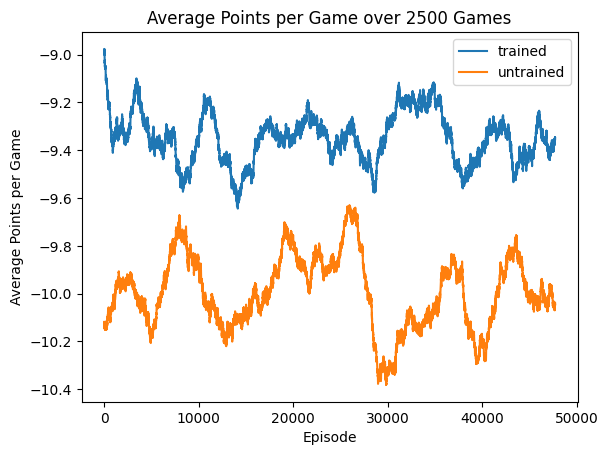
\includegraphics[scale=0.6]{Bilder/points_trained_vs_untrained.png}
    \caption{Durchschnitt der erreichten Punkte pro Spiel }
    \label{fig:untrained_points}
\end{figure}
\begin{figure}[!h]
    \centering
    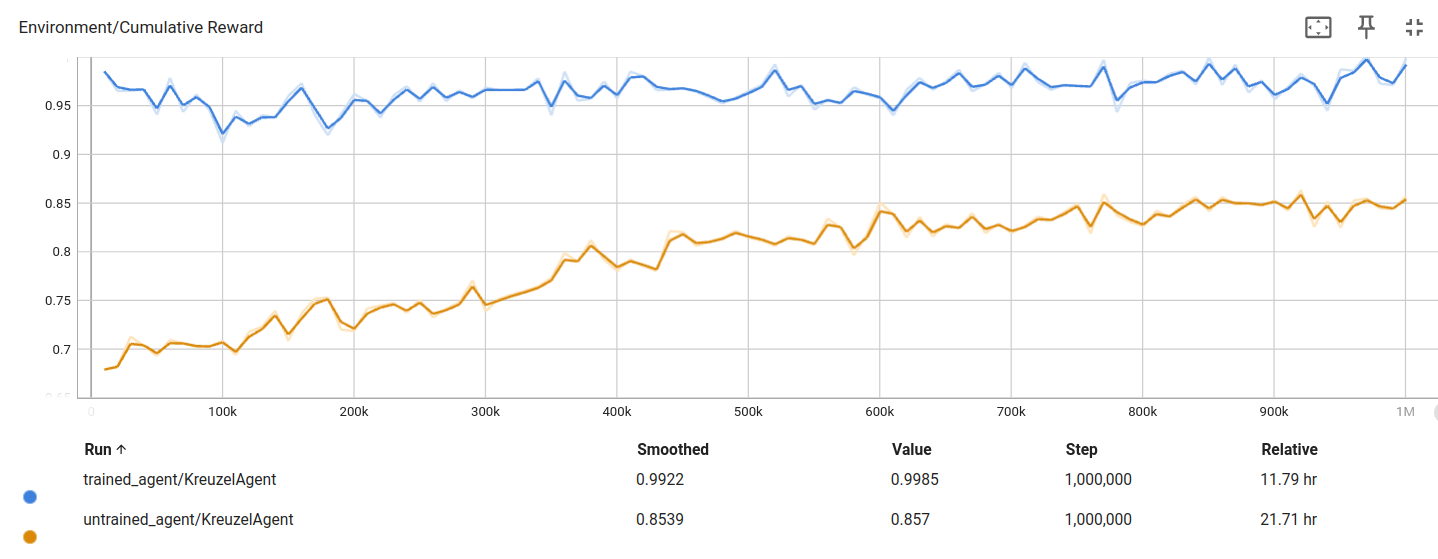
\includegraphics[scale=0.3]{Bilder/rewards_untrained.png}
    \caption{Übersicht der gesammelten Belohnungen}
    \label{fig:untrained_rewards}
\end{figure}

\newpage
\subsection{Trainiert vs Training mit Sonderfeldern}
In diesem Experiment wurden die erreichten Puntke und Rewards des trainierten Agenten gegenüber einem Agenten, welcher mit Sonderfeldern trainiert wurde gegenüber gestellt. \ref{fig:specialFields} stellt den Aufbau der Lernumgebung für das Training dar. Diese speziellen Felder waren einheitlich in die verschiedenen Farben eingefärbt bzw jedes Feld wurde mit Sternfeldern versehen. Dies sollte dazu führen, dass der Agent besser zuweisen kann welche Stellen im Observationsvektor für welche Information zuständig sind. 

\begin{figure}[!h]
    \centering
    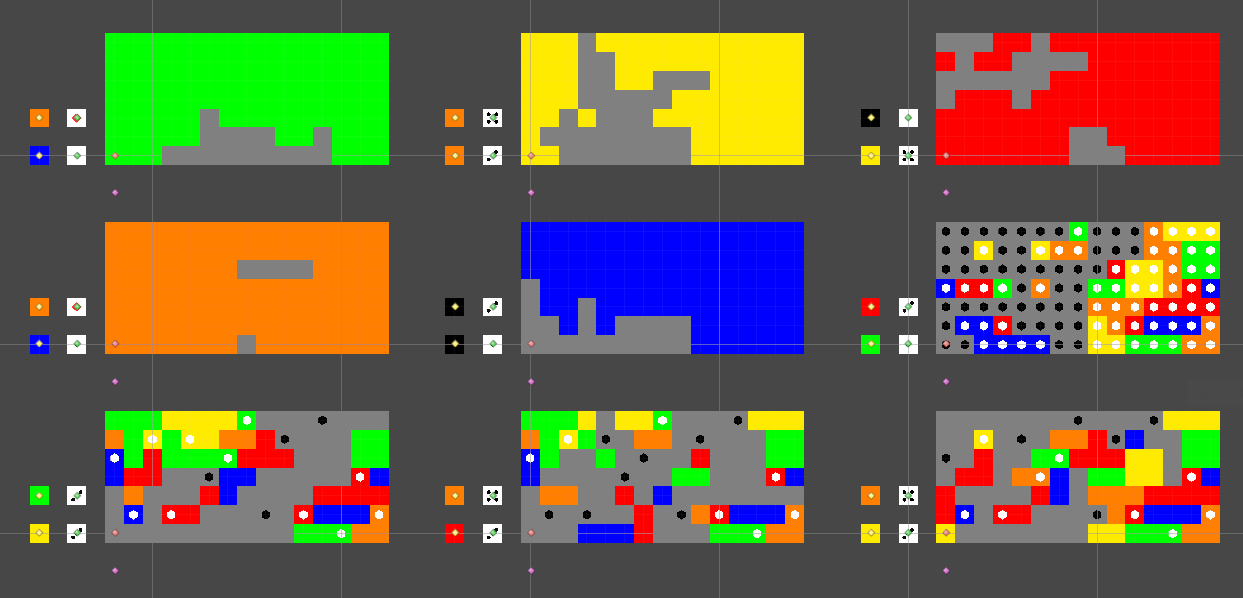
\includegraphics[scale=0.4]{Bilder/specialFields.png}
    \caption{Übersicht der speziellen Felder}
    \label{fig:specialFields}
\end{figure}

In der Grafik \ref{fig:specialFields} ist das Training mit den speziellen Feldern dargestellt. Jedes der Feld hat gewisse Besonderheiten, welche sich zu den normalen Spielfeldern abgrenzen.
Fünf Felder sind in einer kompletten Farbidentität eingefärbt. Hierbei wurde der Zahlenwürfel manipuliert \textbf{<verweis auf Würfelshift>} um häufiger die entsprechende Farbe zu werfen. Diese Felder sollten dem Agenten besser den Zusammenhang des Farbwürfels und des gewählten Farbidentität der Kästchen näherbringen.
In dem anderen Spielfeld ist jedes Feld als Sternfeld markiert. Dies sollte dem Agenten zeigen, dass jedes Feld mit markierten Sternen mehr Punkte bringt.
Bei den anderen drei Feldern ist jedes Feld von vorn herein als verfügbar markiert. Dies sollte zum einen das Konzept des verfügbaren Feldes vermitteln zum anderen dem Agenten ermöglichen das Feld weiter als normal zu explorieren, um die komplexen Ziele des Spiels leichter zu erreichen.
Das Training mit speziellen Feldern führte zu einer Verschlechterung des Ergebnisses wie die nachfolgenden Grafiken zeigen.


\begin{figure}[!h]
    \centering
    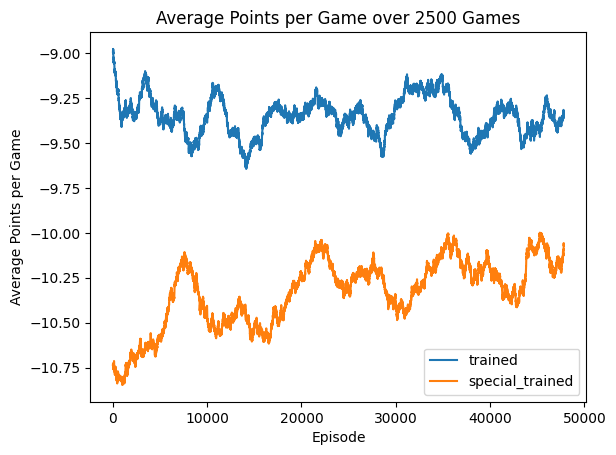
\includegraphics[scale=0.6]{Bilder/points_special_trained.png}
    \caption{Durchschnitt der erreichten Punkte beider Agenten}
    \label{fig:special_points}
\end{figure}


Aus der Grafik \ref{fig:special_points} lässt sich ableiten, dass das Modell welches mit speziellen Feldern trainiert wurde im Durchschnitt weniger Punkte erhalten hat als der normal trainierte Agent.
Dieses Training führte nicht zu einer Verbesserung des Modells. Ursache hierfür liegt sicher im Spielffeld in welchem alle Felder als Sternfelder markiert wurden. Hier konnte der Agent willkürlich Züge ausführen und bekam überdurchschnittlich viele Punkte. Deshalb priorisierte der Agent nicht mehr die eigentlichen Ziele, was wiederum zur Folge hatte, dass die Leistung des Agenten auf dem eigentlichen Feld schlechter wurde. 

\subsection{Trainiert vs Training mit mehr Spielzügen}

In diesem Experiment trainierte der Agent mit mehr zur Verfügung stehenden Spielzügen. Dadurch konnte der Agent das Feld besser explorieren und insgesamt mehr Aktionen auslösen welche zu Belohnungen führten. Dies hat zur Folge, dass auch schwierig erreichbare Rewards ausgelöst wurden, welche somit vom Agent erlernt werden konnten. 
Die Grafik \ref{fig:turns_points} zeigt, dass das Experiment eine Verbesserung des Models zur Folge hatte. Da im Durchschnitt mehr Punkte erreicht wurden.

\begin{figure}[!h]
    \centering
    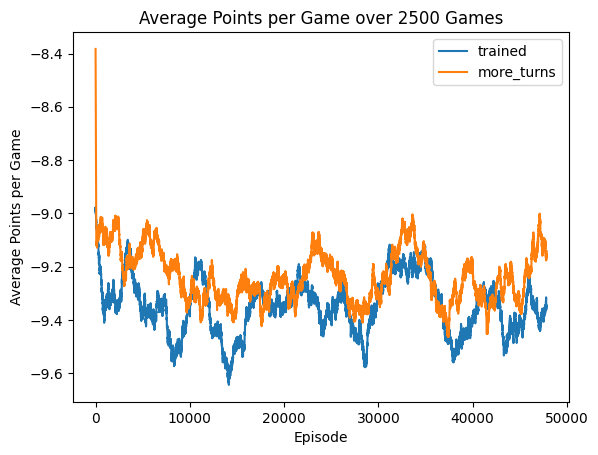
\includegraphics[scale=0.6]{Bilder/points_more_turns.png}
    \caption{Vergleich 'Mehr Züge' und 'trainierter Agent'}
    \label{fig:turns_points}

\end{figure}


\subsection{Überprüfung auf Overfitting}
In diesem Experiment, sollte der Agent auf Overfitting überprüft werden. trainierte und untrainierter Agent spielten das Spiel nach normalen Spielregeln auf einem anderen Spielfeld.
In den Grafiken \ref{fig:orange_points} und \ref{fig:orange_rewards} ist erkennbar, dass beide Agenten ungefähr die selben Rewards gesammelten haben. Der untrainierte Agent konnte im Durchschnitt jedoch etwas mehr Punkte sammeln.
Dies schließt darauf, dass der Agent tatsächlich nur auf dem im Training verwendeten Spielfeld gut performen kann und neue Spielfelder erst erlernen muss.
Interessant ist weiterhin, dass der Durchschnitt aller Punkte etwa 2 Punkte über dem des anderen Spielfeldes liegt, was auf eine höhere Schwierigkeit des schwarzen Spielfeldes hinweist.


\begin{figure}[!h]
    \centering
    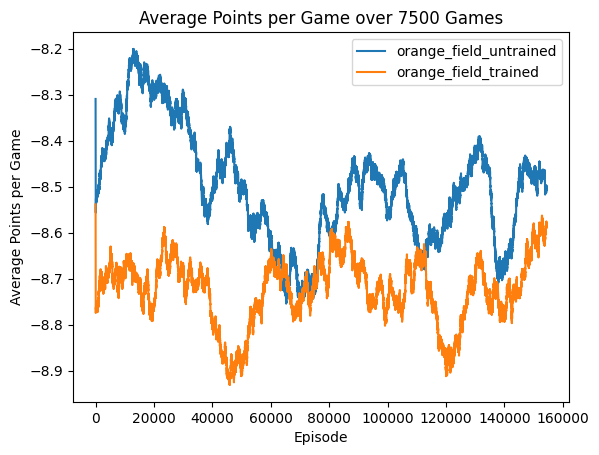
\includegraphics[scale=0.6]{Bilder/points_orange_field.png}
    \caption{Vergleich Punkte 'trainiert' und 'untrainiert' auf orangen Spielfeld}
    \label{fig:orange_points}
\end{figure}
\begin{figure}[!h]
    \centering
    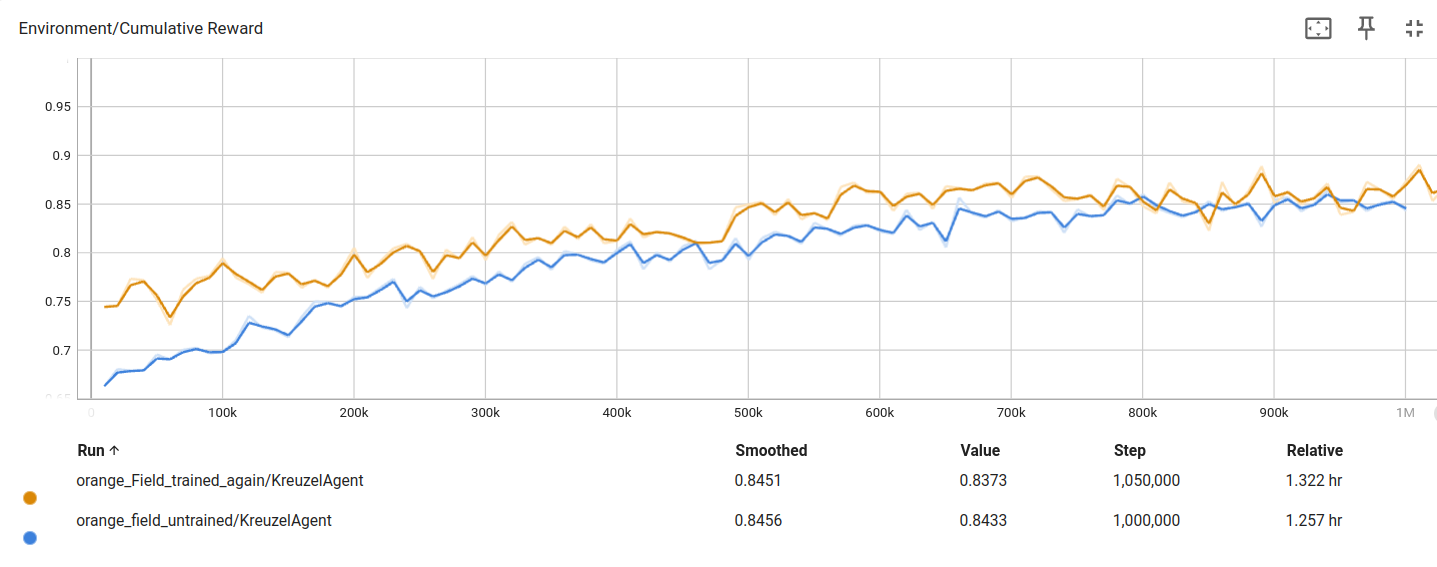
\includegraphics[scale=0.3]{Bilder/rewards_orange_field.png}
    \caption{Übersicht gesammelte Rewards auf orangen Spielfeld}
    \label{fig:orange_rewards}

\end{figure}

\subsection{Training auf Minifeld}
Um zu Überprüfen, ob ein kleineres Feld \textbf{Verweis auf Minifeld.png} einen positiven Effekt auf das Training hat, habe ich bei einem Spielfeld 3 Zeilen abgeschnitten und ließ einen Agenten darauf trainieren.
Im Anschluss überprüfte ich die Leistung des Agenten auf dem normalen Spielfeld gegenüber einem untrainierten Agenten. Da die Observations von Modellen gleich bleiben müssen, entscheid ich mich nicht mehr vorhandene Kästchen mit Nullen im Vektor zu präsentieren. \textbf{Verweis auf auffüllen von leeren feldern}

\begin{figure}[!h]
    \centering
    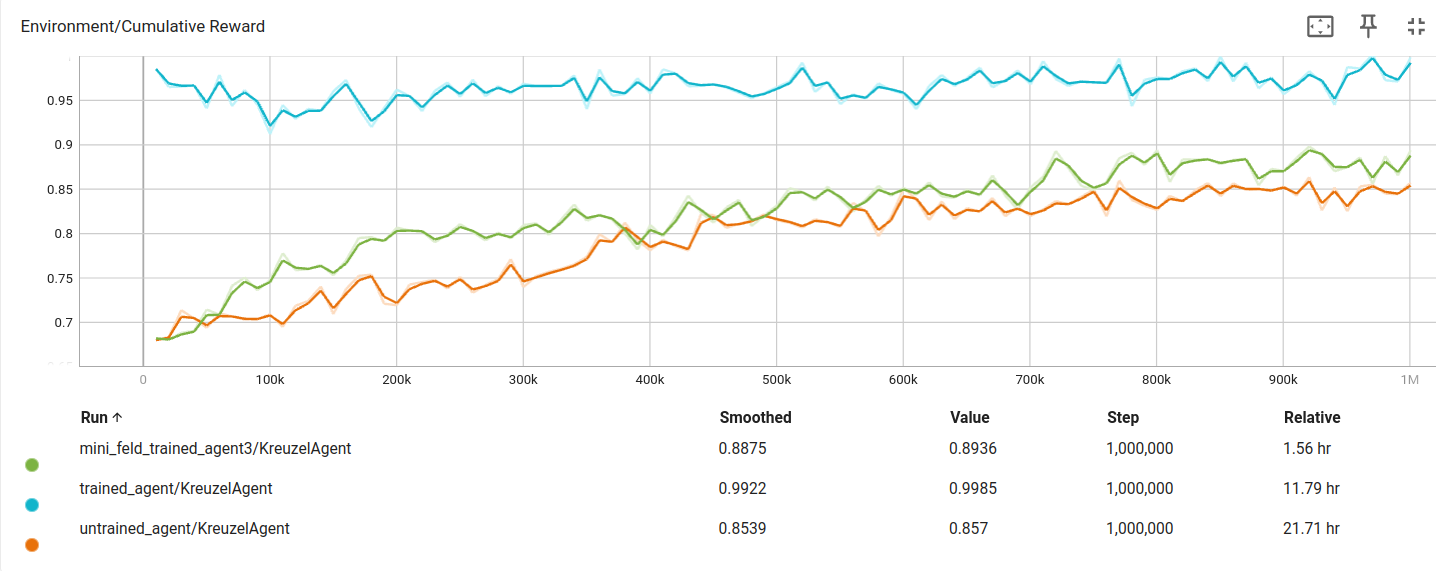
\includegraphics[scale=0.3]{Bilder/rewards_minifield.png}
    \caption{Gesammelte Belohnungen mit Minifeld}
    \label{fig:Minifeld_rewards}
\end{figure}

\begin{figure}[!h]
    \centering
    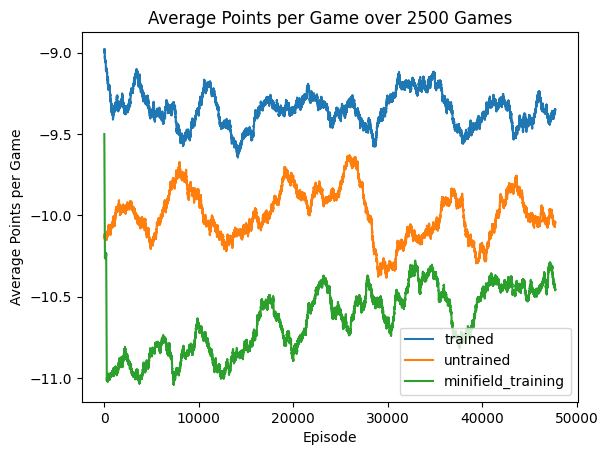
\includegraphics[scale=0.5]{Bilder/points_minifeld.png}
    \caption{Vergleich erreichte Punkte}
    \label{fig:Minifeld_points}
\end{figure}

Die Grafiken \ref{fig:Minifeld_rewards} und \ref{fig:Minifeld_points} zeigen, den Durchschnitt der erreichten Punkte pro Spiel und die gesammelten Blohnungen während des Trainings.
Es wird ersichtlich, dass der mit einem kleinen Feld vortrainierte Agent schlechter performt, als die beiden anderen. Belohnungen wurden auch hier nur verteilt, wenn es zur Punktewertung kommt. Deshalb ist es interessant, dass der untrainierte Agent mehr im Durchschnitt Punkte bekommt, als der auf dem kleinen Feld vortrainierte Agent, obwohl dieser wiederum einen höheren Durchschnitt an Belohnungen erhält. 


\subsection{Training Auswahl KoordinatenPicker}
Da der Agent keine großen Fortschritte erzielen konnte, entschied ich den Agenten das erste Feld durch Koordinaten zu wählen.
Dies setzte Vorraus, dass die Koordinaten der einzelnen Felder in die Observations mit aufgenommen werdne musste und die Observations noch größer wurden.
Damit der Agent lernen kann, welche Koordinaten zu welchen Feldern gehören, entschied ich mich dazu ihn auf einem Spielfeld trainieren zu lassen, wo alle Teilfelder verfügbar sind.
Rewards wurden vergeben für Valide ausgewählte Felder, in Abhängigkeit der gewürfelten Zahlen.

Im nächsten Schritt wird dieses vortrainierte NN genutzt um das Spiel mit richtigen Regeln zu spielen.



\subsection{Training blinder Agent}
In diesem Experiment bekam der Agent lediglich die Würfel, die Anzahl der verbleibenden Joker und die aktuelle Runde des Spiels übergeben.
Dieser Versuch sollte überprüfen, wie gut ein Agent der das aktuelle Spielfeld nicht sieht perfomt. Da die Auswahl der Felder durch mehr oder weniger zufällige Interpolation aller möglichen Felder abläuft, kann der Agent dennoch normal spielen. Durch den Versuchaufbau veringert sich der Beobachtungsvektor von 916 auf eine Größe von 15 Informationen. Dies führte dazu, dass der Agent schnell zu seiner optimalen Policy gelangen konnte. Auch wenn der Agent das Spielfeld nicht sieht, kann er dieses implizit erlernen. Dieser Prozess wäre allerdings nicht sonderlich robust, wäre sehr Lernintensiv und würde nicht auf anderen Feldern funktionieren. Der Agent konnte bereits nach sehr kurzer Zeit von etwa 400k Lernschritten gegen sein Maximum konvergieren, wie in \ref{fig:onlydice_rewards} ersichtlich ist. Dort schneiden sich die beiden grünen Graphen und verbleiben auf ungefähr dem selben Niveau. Dieses Modell wurde insgesamt 5 Mio. Episoden trainiert. Der trainierte Agent konnte sich dagegen kontinuierlich minimal Verbessern. \\
Abbildung \ref{fig:onlydice_points} zeigt, dass auch der blinde Agent, im Durchschnitt weniger Punkte erreichen konnte. Dies beweist, dass das Training trotz der geringen erreichten Punkte positiv verlaufen ist.


\begin{figure}[!h]
    \centering
    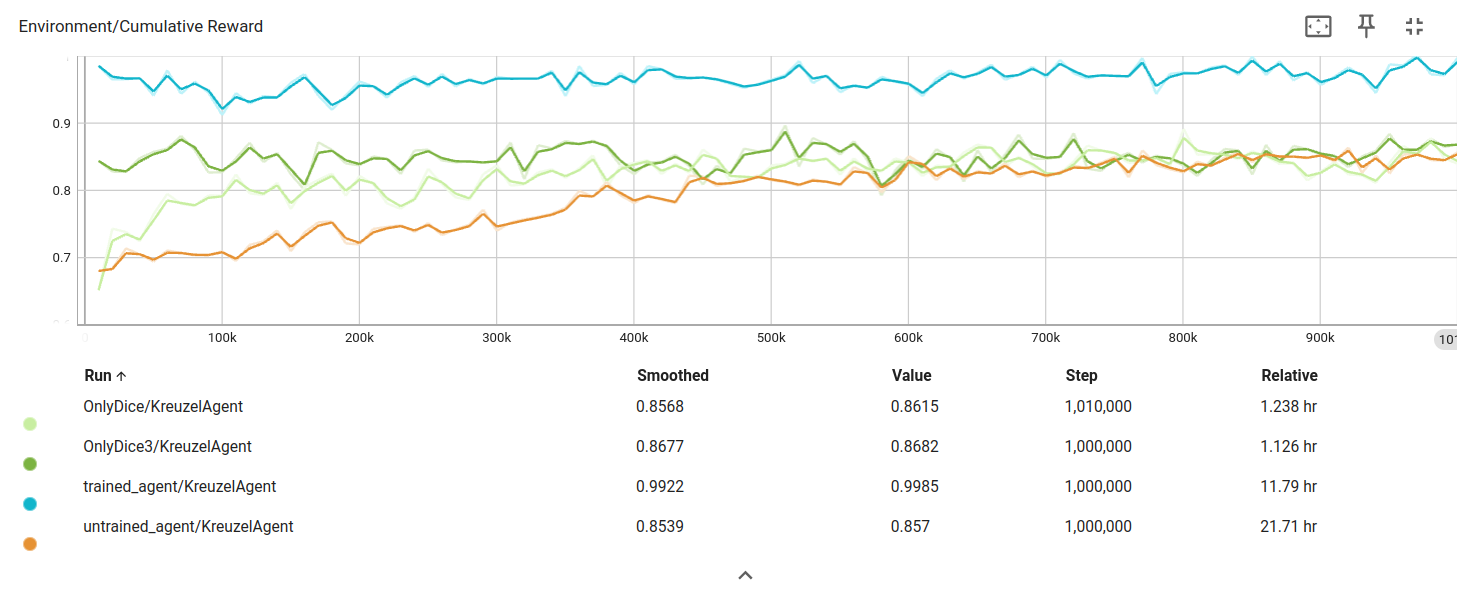
\includegraphics[scale=0.3]{Bilder/rewards_onlydice.png}
    \caption{Gesammelte Belohnungen blinder Agent}
    \label{fig:onlydice_rewards}
\end{figure}

\begin{figure}[!h]
    \centering
    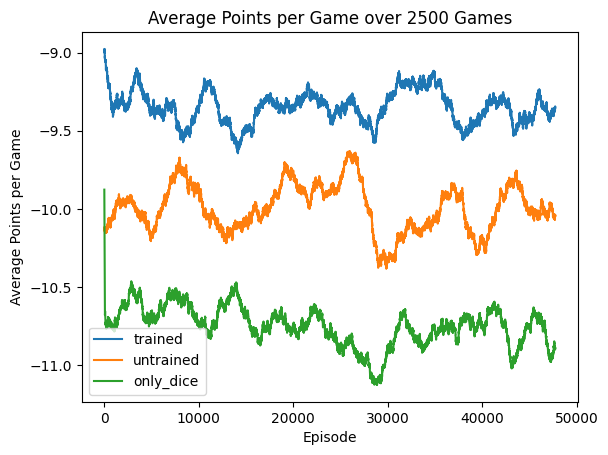
\includegraphics[scale=0.5]{Bilder/points_onlydice.png}
    \caption{Vergleich erreichte Punkte blinder Agent}
    \label{fig:onlydice_points}
\end{figure}